% !TeX encoding   = UTF-8
\documentclass[msc,proposal,hidelot,hideabstract]{ppgccufmg} % ou [msc] para dissertações
                                        % de mestrado. Para propostas ou
                                        % projetos, usar [phd,project],
                                        % [msc,proposal], etc.
\usepackage[brazil]{babel} % ajusta vários detalhes para
                           % documentos escritos em português,
                           % principalmente hifenização
\usepackage[T1]{fontenc}   % permite a hifenização de
                           % palavras acentuadas
\usepackage[utf8x]{inputenc} % ou [utf8x] para quem prefere
                             % usar a codificação UTF-8
\usepackage{graphicx} % define o comando \includegraphics
                      % para a inclusão de Figuras
%\usepackage[square]{natbib} % permite citações naturalmente
                            % integradas ao texto
\usepackage[a4paper,
portuguese,
bookmarks=true,
bookmarksnumbered=true,
linktocpage,
colorlinks=true,
citecolor=black,
urlcolor=black,
linkcolor=black,
filecolor=black,
]{hyperref}
\usepackage[table,xcdraw]{xcolor}
\usepackage{amsmath}

\usepackage{todonotes}
\begin{document}
\ppgccufmg{
title={Um Estudo de Ferramentas de \\
Gerenciamento de Requisição de Mudança},
author={Vagner Clementino dos Santos},
university={Universidade Federal de Minas Gerais},
course={Ciência da Computação},
address={Belo Horizonte},
date={2016-06},
advisor={Rodolfo F. Resende},
%abstract={Resumo}{resumo},
}
\chapter{Introdução}
\label{ch:intro}
Dentro do ciclo de vida de um produto de software o processo de manutenção tem
papel fundamental. Devido ao seu alto custo, em alguns casos chegando em 60\%
do preço final do software \cite{kaur2015review}, a atividade relacionadas a manter e evoluir software vem tendo sua importância considerada tanto pela comunidade científica quanto pela indústria.

\textit{Manutenção} pode ser definida como o processo de modificar um componente ou sistema de software após a sua entrega com o objetivo de \textit{corrigir falhas, melhorar o desempenho ou adaptá-lo devido à mudanças ambientais} \cite{{159342}}. De outra forma, \textit{Manutenibilidade} é a propriedade de um sistema ou componente de software com relação ao grau de \textit{facilidade}
em que ele pode ser corrigido, melhorado ou adaptado \cite{{159342}}.

As manutenções em software podem ser divididas em \textit{Corretiva, Adaptativa, Perfectiva e Preventiva} \cite{Lientz:1980:SMM:601062,159342}. A Manutenção Corretiva lida com a reparação de falhas encontradas. A Adaptativa tem o seu foco na adaptação do software devido à mudanças ocorridas no ambiente em que ele está inserido. A Perfectiva trabalha com a modificação de um produto de software com o objetivo de detectar e corrigir falhas latentes antes que elas se manifestem como tal. A  Perfectiva fornece melhorias na documentação, desempenho ou manutenibilidade do sistema. A Preventiva se preocupa com atividades que possibilitem aumento da manutenibilidade do sistema. A \textit{ISO 14764} \cite{1703974} propõe a divisão da tarefa de manutenção nos quatro tipos descritos anteriormente e agrupa-os em termo único denominado \textit{Requisição de Mudança - Modification Request (RM)}, conforme pode ser visto pela Figura \ref{fig:modification-request}

\begin{figure}[hbtp]
\centering
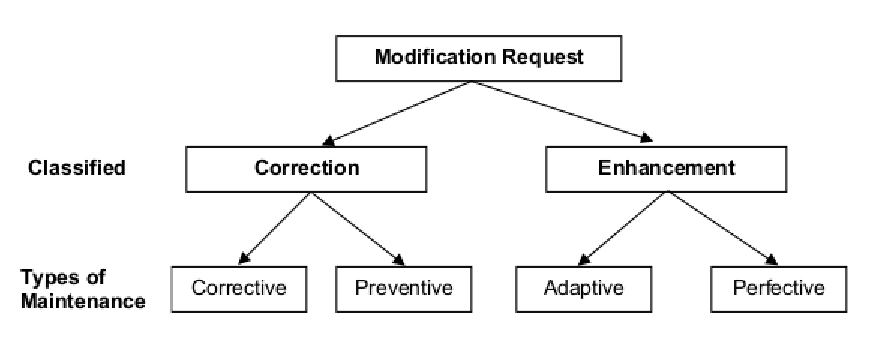
\includegraphics[width=.75\textwidth]{../img/modification_request.eps}
\caption{Tipos de manutenção segundo a norma ISO/IEC 14764. Extraído de
  \cite{1703974}}
\label{fig:modification-request}
\end{figure}

Em um ambiente real de desenvolvimento e manutenção de software, independente do tipo
de Requisição de Mudança, existe a necessidade de que ela seja gerenciada, especialmente por conta do seu volume. Esse controle é geralmente realizado por Sistemas de Controle de Demandas (SCD)- Issue Tracking Systems  que ajudam
os desenvolvedores na correção de forma individual ou colaborativa de defeitos (bugs), bem como no desenvolvimento de novas funcionalidades. Verifica-se na literatura diversos
sinônimos para os Sistemas de Controle de Demanda (Sistema de Controle de
Defeitos - Bug Tracking Systems, Sistema de Gerenciamento da Requisição -
Request Management System e outros ), todavia, de modo geral, o
termo se refere as ferramentas utilizadas pelas organizações para \textit{gerenciar as Requisições de Mudança}. Os SCD's podem ainda serem utilizados por gestores, analistas de qualidade e usuários finais para atividades tais como gerenciamento de projetos, comunicação, discussão e revisões
de código.

A maioria desses sistemas são projetados em torno do termo "demanda"
(bug, defeito, bilhete, recurso, etc.), contudo, cada vez mais este modelo parece
ser distante das necessidades práticas dos projetos de software. No trabalho de Baysal e outros \cite{Baysal:2013:SAP:2486788.2486957} revelou com desenvolvedores enfrentam dificuldades para manter uma compreensão global das demandas no qual estão envolvidos (impacto, relação com outros módulos ou demandas e etc.). Apesar da crescente importância dos SCD's, percebe-se um aparente desacoplamento com as necessidades dos diversos interessados(stakeholders) na manutenção e evolução de software. Um sinal deste distanciamento pode ser observado pelas diversas extensões (plugins) propostas na literatura \cite{101186,Thung:2014:BIT:2635868.2661678,Kononenko:2014:DED:2591062.2591075}.

A manutenção de software muitas vezes aparece ligada aos processos tradicionais
de desenvolvimento de software. Existe o mito de que os métodos ágeis estão
principalmente concentrados na fase de desenvolvimento
\cite{kajko2009model}. No entanto, especialistas em software cada vez mais
avaliam que práticas ágeis podem ser adaptadas à evolução do software. Isso não
é totalmente surpreendente, já que métodos ágeis enfatizam a importância das
pessoas, o desenvolvimento incremental, a redução de riscos e teste contínuo. Todos estes fatores contribuem para a evolução e manutenção de um software
\cite{thomas2006agile}. Desta forma tanto em um contexto que utilize processo de manutenção
``tradicional'' ou em que se aplique métodos ágeis pode-se tirar proveito das
FGRM's para um melhor desempenho das atividades de manutenção.

Neste trabalho de dissertação vamos estudar as Ferramentas de Gerenciamento de Requisição de Mudança (FGRM) como o objetivo de \textit{(i)} entender as funcionalidades comuns deste tipo de ferramenta; \textit{(ii)} mapear as extensões para as FGRM's que estão sendo propostas na literatura; \textit{(iii)} avaliar sobre o ponto de vista dos profissionais a situação atual das FGRM; \textit{(iv)} propor novas extensões para as FGRM.
	
Esta proposta de dissertação está estruturada da seguinte forma: o  Capítulo
\ref{ch:justificativa} discute a relevância deste trabalho no contexto da Engenharia de Software, em especial no processo de Manutenção de Software. O Capítulo \ref{ch:revisao} revisa a literatura com relação aos trabalhos desenvolvidos sobre Manutenção de Software; é dado um foco especial
nos estudos que focam nas FGRM's. No Capítulo \ref{ch:metodologia} é discutida a metologia a ser aplicada visando a elaboração do trabalho. No Capítulo \ref{ch:conclusao_trab_futuros} é apresentado o cronograma de atividades da dissertação através da Tabela \ref{tab:cronograma}.

\chapter{Justificativa}
\label{ch:justificativa}
Desde o final da década de 1970 \cite{Zelkowitz:1979:PSE:578504} percebe-se o aumento do custo referente as atividades de  manutenção de software. Nas décadas de 1980 e 1990 alguns
trabalhos tiveram seu foco no desenvolvimento de modelos de mensuração do custo
para manter o software \cite{Herrin:1985:SMC:323287.323383,hirota1994approach}. Apesar da evolução das metologias da manutenção de software a estimativa é que nas últimas duas décadas o custo de manutenção tenha aumentado em 50\% \cite{koskinen2010software}. Esta tendência pode ser observada na Figura \ref{fig:software-maintence-costs} no qual é possível verificar a evolução do custo da manutenção de software como fração do custo total do produto.

\begin{figure}
\centering
\includegraphics[width=0.7\linewidth]{../img/software-maintence-costs}
\caption{Evolução da manutenção de software como percentual do custo total.	Extraído de	\cite{engelbertink2010save}}

\label{fig:software-maintence-costs}
\end{figure}

Diante da maior presença de software em todos os setores da sociedade
existe um interesse por parte da academia e da industria no desenvolvimento de
processos, técnicas e ferramentas que reduzam o esforço e o custo das tarefas
do desenvolvimento de manutenção. Neste linha, o trabalho de Yong \& Mookerjee \cite{1423995}  propõe um modelo que reduz o custos de manutenção e reposição durante a vida útil de um sistema de software. O modelo demonstrou que em algumas situações é \textit{melhor substituir um sistema do que mantê-lo}. Em outros estudos há menção de que o custo de manutenção pode chegar a 60\% do custo total do software \cite{kaur2015review}. Este mesmo percentual refere-se ao total de desenvolvedores dedicados à tarefas de manutenção de sistemas \cite{Zhang_2003}.

A manutenção não necessariamente exige que o processo de software envolvido
seja o tradicional. Percebe-se alguns exemplos de adoção das práticas ágeis
para fins de manutenção e evolução do software \cite{kajko2009model}. Tal
tendência não é surpreendente tendo em vista que métodos ágeis enfatizam
características úteis à eficiência da implementação de software, tais como desenvolvimento incremental e teste contínuo que agregam valor para a evolução e manutenção eficaz de um sistema
\cite{thomas2006agile}.

O desenvolvimento e a manutenção de software envolvem diversos tipos de métodos,
técnicas e ferramentas. Em especial no processo de manutenção, um aspecto
importante são as diversas Requisições de Mudanças que devem ser
gerenciadas. Este controle é realizado pelas Ferramentas de Gerenciamento de Requisição de Mudanças (FGRM) cujo uso vêm crescendo em importância, sobretudo, por sua utilização por gestores, analistas da qualidade e usuários finais para atividades como tomada de decisão e comunicação, dentre outras.

A utilização de  \textit{``demanda''} como conceito central para Ferramentas de Gerenciamento de Requisição de Mudanças (FGRM) parece ser distante das necessidades práticas dos projetos de software, especialmente no ponto de vista dos desenvolvedores \cite{Baysal:2013:SAP:2486788.2486957}. Um exemplo deste desacoplamento das FGRM com a necessidade de seus usuários pode ser visto no trabalho proposto por Baysal \& Holme \cite{baysal2012qualitative} no qual desenvolvedores que utilizam o Bugzilla\footnote{\url{https://www.bugzilla.org}} relatam a
dificuldade em manter uma compreensão global das RM's em que eles estão
envolvidos. Segundo os desenvolvedores seria interessante que a ferramenta
tivesse um suporte melhorado para a Consciência Situacional - Situational
Awareness. Em síntese, eles gostariam de estar cientes da situação global do
projeto bem como das atividades que outras pessoas estão realizando. Um outro
sinal da necessidade de evolução do deste tipo de ferramenta pode ser observado considerando as diversas extensões (plugins) propostas na literatura \cite{101186,Thung:2014:BIT:2635868.2661678,Kononenko:2014:DED:2591062.2591075}

Neste contexto, é proposto neste projeto de dissertação a elaboração de um estudo das as Ferramentas de Gerenciamento de Requisição de Mudança (FGRM) como o objetivo de \textit{(i)} entender os requisitos comuns deste tipo de ferramenta; \textit{(ii)} mapear as extensões para as FGRM que estão sendo propostas na literatura; \textit{(iii)} avaliar sobre o ponto de vista dos profissionais a situação atual dos FGRM; \textit{(iv)} propor novas extensões para as FGRM. Vamos discutir os aspectos que são
considerados mais importantes a partir da literatura da área bem como dos pontos de vistas de alguns profissionais. De forma particular, iremos estudar os mecanismos de personalização que algumas destas ferramentas permitem e tentaremos ainda criar exemplos de personalização para alguma possível extensão a ser identificada ao longo do trabalho.

\chapter{Revisão da Literatura}
\label{ch:revisao}

Uma tendência natural do software é evoluir a fim de atender aos novos requisitos e alterações no ambiente no qual ele está inserido. Em uma séria de estudos Lehman e outros propõem um conjunto de leis sobre a evolução do software. Dentre elas podemos destacar as leis da Mudança Contínua (Continuing
Change) e da Complexidade Crescente (Increasing complexity). Segundo a lei da
Mudança Contínua um programa que é utilizado em um ambiente real deve mudar ou se tornará progressivamente menos útil \cite{lehman1980understanding}. A lei da
Complexidade Crescente (Increasing complexity) afirma que quando um sistema em
evolução muda, sua estrutura tende a ser tornar mais complexa. Nesta situação,
recursos extras devem ser disponibilizados a fim de preservar e simplificar a
estrutura do software \cite{lehman1980understanding}. As leis de Lehman têm
sido validadas, especialmente aquelas relacionadas a tamanho e
complexidade do software. Em um trabalho recente Yu \& Mishra \cite{{yu2013empirical}} examinaram e avaliaram de forma empírica as Leis de Lehman com relação a evolução da qualidade do software. Os
resultados dão suporte as Leis de Lehman especialmente a que versa sobre a qualidade, na qual um produto de software decresce a sua qualidade ao longo do tempo, exceto que ele seja reestruturado.

Percebida a importância do processo de manutenção de software, alguns trabalhos foram propostos visando mensurar o seu custo bem como propor processos visando a redução do esforço envolvido neste tipo de atividade.

No trabalho de Herrin \cite{Herrin:1985:SMC:323287.323383} foi proposto um modelo matemático com o
objetivo de avaliar o impacto financeiro no orçamento de uma universidade devido às atividades de manutenção no sistema de processamento de dados da instituição. O modelo propõe que o valor disponível para desenvolvimento de um novo sistema é função inversa do custo de manutenção do software existente. Desta forma, o fato de se manter um sistema durante muito tempo poderá impossibilitar a aquisição ou mesmo o desenvolvimento de um novo.

No estudo de Hirota et al. \cite{hirota1994approach} é proposta a utilização da técnica Análise de Ripple para estimar o custo da manutenção de software. O termo ``efeito Ripple'' foi utilizado pela primeira vez em um artigo publicado por Haney \cite{haney1972module} para descrever a forma que a mudança em um módulo poderia causar alterações em outras partes do sistema \cite{bilal2005using}. A Análise Ripple é, portanto, uma técnica de analisar o fluxo de dados de variáveis dentro de um determinado programa. Os valores retornados pela aplicação da técnica são denominados Complexidade de Ripple. Os resultados demostraram que a Complexidade de Ripple está mais relacionada ao entendimento do
software do que as métricas padrão, como linhas de código, complexidade ciclomática e pontos de função. Desta forma, a Complexidade de Ripple poderia ser utilizada, por exemplo, para predizer os custo de manutenção de um sistema, bem como a necessidade de substituição do mesmo.

Mediante o uso de Redes Neurais Shula \& Misra
\cite{Shukla:2008:ESM:1342211.1342232} propõe um estudo para medir o custo de
manutenção de software. O trabalho discute a utilização de outras métricas além
de linha de código e pontos de função para medir  tamanho e custo do processo de manutenção. Os resultados demonstraram a possibilidade de construir um modelo para medir o custo utilizando Redes Neurais. Contudo, os resultados são sensíveis a escolha da arquitetura e parâmetros de treino, os quais idealmente deveriam ser preparados por um especialista no sistema (oráculo).

Diante da crescente importância das Ferramenta de Gerenciamento de Requisição de Mudanças (FGRM) no processo de manutenção de software, diversos trabalhos vêm sendo propostos com o objetivo de entender como elas estão sendo utilizadas bem como sugerir melhorias no desenho para desenvolver futuras FGRM's.

No trabalho de Junio et al. \cite{5741246} é proposto um processo denominado PASM (Process for Arranging
Software Maintenance Requests) que propõe lidar com tarefas de manutenção como projetos de software. Para tanto, utilizou-se técnicas de análise de agrupamento (clustering) a fim de melhor compreender e comparar as demandas de manutenção. Os resultados demostraram que depois de adotar o PASM os
desenvolvedores têm dedicado um tempo maior para análise e validação e menos para tarefas de execução e de codificação, ou seja, realizando tarefas de maior valor agregado.

No estudo realizado por Bettenburg et al. \cite{bettenburg2008makes} foi
desenvolvida uma pesquisa (\textit{survey}) entre desenvolvedores e usuários dos
projetos Apache\footnote{\url{http://www.apache.org/}}, Eclipse\footnote{\url{https://www.eclipse.org}} e Mozilla\footnote{\url{https://www.mozilla.org}} a fim de verificar o que
produziria uma boa FGRM. Os resultados demonstraram que do ponto de vista dos desenvolvedores foram consideradas úteis funcionalidades tais como reprodução do erro, rastros de pilhas (stack traces) e casos de testes. A partir deste resultado foi construído um protótipo capaz de conduzir os usuários na coleta e fornecimento de um maior número de informações úteis para a resolução do defeito reportado.

Avaliando o controle de demandas como um processo social, Bertram et
al. \cite{Bertram:2010:CCB:1718918.1718972} realizaram um estudo qualitativo em
FGRM's quando utilizados por pequenas equipes de desenvolvimento de software. Os resultados mostraram que este tipo ferramenta não é apenas um banco de dados de rastreamento de defeitos, recursos ou pedidos de informação, mas também atua como um ponto focal para a comunicação e coordenação para diversas partes interessadas (stakeholders) dentro e fora da equipe de software. Os
clientes, gerentes de projeto, o pessoal envolvido com a garantia da qualidade
e programadores, contribuem em conjunto para o conhecimento compartilhado dentro do contexto das FGRM's.

Em Zimmermann et al. \cite{5070993} é discutido a importância de que a informação descrita em uma Requisição de Mudança seja relevante e completa a fim de que o defeito reportado seja resolvido rapidamente. Contudo, na prática, a informação apenas chega ao desenvolvedor com a qualidade requerida após diversas interações com o usuário afetado. Com o objetivo de minimizar este
problema os autores propõe um conjunto de diretrizes para a construção de um ferramenta capaz de reunir informações relevantes a partir do usuário e identificar arquivos que precisam ser corrigidos para resolver o defeito.

No trabalho de Breu et al.\cite{Breu:2010:INB:1718918.1718973} o foco é analisar o papel dos FGRM's no suporte à colaboração entre desenvolvedores e usuários de um software. A partir da análise quantitativa e qualidade de uma amostra de defeitos registrados em uma FGRM de dois projetos de software livre, foi possível verificar que os usuários desempenham um papel além de simplesmente reportar uma falha: a participação ativa e permanente dos usuários finais foi importante no progresso da resolução das falhas que eles descreveram.

O desenvolvimento de novas funcionalidades em FGRM's, mediante a capacidade de
extensão propiciada por algumas delas vêm sendo explorada na literatura. \textit{Buglocalizer} \cite{Thung:2014:BIT:2635868.2661678} é uma extensão para o Bugzilla que possibilita a localização dos arquivos do código fonte que estão relacionados ao defeito relatado. A ferramenta extrai texto dos campos de sumário e descrição de um determinado erro reportado no Bugzilla. Este texto é comparado com o código fonte através de técnicas de Recuperação da Informação.

\textit{NextBug} \cite{101186} é uma extensão para o Bugzilla que
recomenda novos bugs para um desenvolvedor baseado no defeito que ele esteja
tratando atualmente. O objetivo da extensão é sugerir defeitos com base em técnicas de
Recuperação de Informação.

No trabalho de Kononenko et al. \cite{Kononenko:2014:DED:2591062.2591075} é
apresentada uma ferramenta denominada \textit{DASH} cujo objetivo é agrupar as
demandas que são relevantes para as atividades de um desenvolvedor. Naturalmente todas as demandas ditas relevantes deveriam estar sob a responsabilidade de um mesmo programador. O principal objetivo desta ferramenta é aumentar a Consciência Situacional (Situational Awareness) dos
desenvolvedores. Segundo os autores, o principal ganho do uso da ferramenta é
que os programadores podem gerenciar melhor o excesso de informação e ficar
mais ciente da evolução das demais demandas do sistema.

Na ferramenta proposta por Thung et al. \cite{Thung:2014:DIT:2642937.2648627} o
foco é na determinação de defeitos duplicados. A contribuição deste trabalho é a
integração do estado da arte de técnicas não supervisionadas para detecção de
falhas duplicadas conforme proposto por Runeson et al. \cite{Runeson:2007:DDD:1248820.1248882}. A ferramenta utiliza o Modelo de Vetor Espacial (Vetor Space Model) como métrica de similaridade entre os defeitos e fornece aos desenvolvedores uma lista de possíveis duplicatas.

\chapter{Metodologia}
\label{ch:metodologia}

O trabalho de dissertação proposto pode ser dividido nas etapas listadas a seguir:


	\begin{itemize}[(i)]
		\item Mapeamento Sistemático da Literatura \cite{keele2007guidelines}
		\item Caracterização das Ferramentas de Gerenciamento de Requisição de Mudança (FGRM)
		\item Pesquisa (Survey) com os desenvolvedores \cite{wohlin2012experimentation}
		\item Desenvolvimento de extensões para as FGRM's
	\end{itemize}

Nas próximas seções iremos detalhar cada uma das etapas que compõem o trabalho de dissertação proposto.

\section{Mapeamento Sistemático da Literatura}
\label{sec:revisao_sistematica}

Um \textit{Mapeamento Sistemático da Literatura}, também conhecido como Estudos de Escopo (Scoping Studies), tem como objetivo fornecer uma visão geral de determinada área de pesquisa, estabelecer se existem evidências de estudos sobre determinado tema e fornecer uma indicação da quantidade de trabalho na linha de pesquisa sob análise \cite{keele2007guidelines,wohlin2012experimentation}. Na dissertação a ser realizada será utilizado as diretrizes proposta \cite{keele2007guidelines} no qual o Mapeamento deve seguir os seguintes passos:

\begin{enumerate}
  \item \textbf{Planejamento}
  \begin{enumerate}
    \item \textit{Identificar a necessidade da Revisão}
    \item \textit{Especificar questões de pesquisa}
    \item \textit{Desenvolver o Protocolo da Revisão}
  \end{enumerate}
  \item \textbf{Condução/Execução}
  \begin{enumerate}
    \item \textit{Seleção dos Estudos Primários}
    \item \textit{Análise da qualidade dos Estudos Primários}
     \item \textit{Extração dos Dados}
     \item \textit{Sintetização dos Dados}
   \end{enumerate}
  \item \textbf{Escrita/Publicação}
  \begin{enumerate}
    \item \textit{Redigir documento com os resultados da Revisão}
    \item \textit{Redigir documento com lições aprendidas}
  \end{enumerate}
\end{enumerate}

O mapeamento será conduzido com o objetivo de responder as questões de pesquisas propostas a seguir. Com estas respondas espera ser possível ter uma visão mais abrangente da linha de pesquisa estudada. Além disso, o mapeamento será utilizado na elaboração de uma pesquisa com desenvolvedores (vide Seção \ref{sec:survey}) e na proposição de novas extensões para as FGRM.

\begin{itemize}
  \item \textbf{$Q1$}: Quais são as funcionalidades propostas para estender as FGRM?
  \item \textbf{$Q2$}: Qual técnica foi utilizada para desenvolver a extensão?
  \item \textbf{$Q3$}: Quais as FGRM estão sendo estendidas?
  \item \textbf{$Q4$}: Como foi realizado o processo de avaliação da extensão proposta?
\end{itemize}


\section{Caracterização dos requisitos das Ferramentas de Gerenciamento de Requisição de Mudança}
\label{sec:caracterizacao}

Esta etapa do trabalho consistirá de um estudo exploratório com o objetivo de determinar quais são as funcionalidades comuns às Ferramentas de Gerenciamento de Requisição de Mudança (FGRM). O estudo consistirá na leitura da documentação de alguns FGRM para que de forma sistemática seja levantado quais são as funcionalidades oferecidas por determinada ferramenta. O método de escolha das FGRM será avaliado posteriormente, todavia, um possível ponto de partida é a lista disponível na Wikipedia que compara diversas FGRM\footnote{\url{https://en.wikipedia.org/wiki/Comparison_of_issue-tracking_systems}}.

O resultado deste estudo permitirá compreender melhor este tipo de ferramenta tomando como base as suas funcionalidades em comum. Também será possível propor extensões para as FGRM (Seção ref{sec:novas-extensoes}) tendo em vista a possibilidade de determinar o conjunto mínimo de funções deste tipo de sistema. 

\section{Pesquisa com Profissionais}
\label{sec:survey}
Com o objetivo de coletar os aspectos mais importantes das FGRM's do ponto de
vista dos profissionais ligados à manutenção de software será realizada uma
 pesquisa (survey). O planejamento e o desenho da pesquisa seguirá as diretrizes propostas em \cite{wohlin2012experimentation}.

A população da pesquisa proposta é a comunidade envolvida com o processo de
manutenção de software e que faça uso de FGRM's. Neste contexto, seriam
possíveis amostras, os desenvolvedores envolvidas com tarefas de manutenção nos
projetos da Mozilla\footnote{\url{https://bugzilla.mozilla.org/}} ou da
Eclipse Foundation\footnote{\url{https://bugs.eclipse.org/bugs/}}. Durante a
execução da dissertação será avaliado qual amostra caracteriza melhor a
população do estudo.

\section{Extensões para Ferramentas de Gerenciamento de Requisição de Mudança}
\label{sec:novas-extensoes}

A partir dos resultados do Mapeamento Sistemática, do Estudo de Caracterização das ferramentas e da Pesquisa com o profissionais pretende-se desenvolver uma ou mais extensão (plugin) para determinada FGRM. Cabe ressaltar que esta parte do trabalho será realizada caso o esforço seja compatível com os prazos e recursos disponíveis. No caso da implementação de um plugin este será apresentado e avaliado mediante a realização de um \textit{Experimento Controlado} \cite{wohlin2012experimentation} utilizando a base de dados de demandas de manutenção de uma empresa de software real. Este experimento será conduzido com o objetivo de avaliar a utilização de uma extensão em um ambiente de desenvolvimento e manutenção de software real. Os dados serão coletados tomando os ponto de vistas dos desenvolvedores.

\chapter{Conclusão e Trabalhos Futuros}
\label{ch:conclusao_trab_futuros}

A Manutenção de Software é um processo complexo e caro e, portanto,  merece atenção da
comunidade acadêmica e da indústria. Desta forma, emerge a necessidade do desenvolvimento de técnicas, processo e ferramentas que reduzam o custo e o esforço envolvidos nas atividades de manutenção e evolução de software. Neste contexto, as Ferramentas de Gerenciamento de Requisição de Mudança desempenham um papel fundamental que ultrapassa a simples função de registrar falhas em software. Neste sentido é proposto o estudo para entender o papel desta ferramenta, analisar a literatura sobre o assunto e discutir os aspectos que são considerados mais importantes do ponto de vista dos profissionais. As atividades para atingir o objetivo da dissertação são exibidas de forma macro na Tabela \ref{tab:cronograma}. No desenvolvimento da dissertação será realizado um
cronograma mais detalhado das atividades.
% Please add the following required packages to your document preamble:
% \usepackage{graphicx}
\begin{table}[]
	\label{tab:cronograma}
	\centering
	\resizebox{\textwidth}{!}{%
		\begin{tabular}{|l|l|c|c|}
			\hline
			\multicolumn{4}{|c|}{\textbf{CRONOGRAMA DISSERTAÇÃO}}                                                                                                                 \\ \hline
			\# & \multicolumn{1}{c|}{\textbf{Atividade}}                                               & \textit{\textbf{Início (MM/AAAA)}} & \textit{\textbf{Término (MM/AAAA)}} \\ \hline
			01 & Mapeamento  Sistemático da Literatura                                                 & \textit{03/2016}                   & \textit{06/2016}                    \\ \hline
			02 & Ponto de Controle 01 – Reunião com orientador sobre Revisão Sistemática da Literatura & \textit{06/2016}                   & \textit{06/2016}                    \\ \hline
			03 & Caracterização das Ferramentas de Gerenciamento de Requisição de Mudança              & \textit{06/2016}                   & \textit{07/2016}                    \\ \hline
			04 & Ponto de Controle 02 – Reunião com orientador sobre a Caracterização das FGRM           & \textit{07/2016}                   & \textit{07/2016}                    \\ \hline
			05 & Pesquisa com Profissionais                                                            & \textit{08/2016}                   & \textit{09/2016}                    \\ \hline
			06 & Ponto de Controle 03 – Reunião com orientador sobre a Pesquisa com o Profissionais    & \textit{09/2016}                   & \textit{09/2016}                    \\ \hline
			07 & Implementação da Ferramenta                                                           & \textit{09/2016}                   & \textit{10/2016}                    \\ \hline
			08 & Ponto de Controle 03 – Avaliação da Ferramenta Avaliada                               & \textit{10/2016}                   & \textit{10/2016}                    \\ \hline
			09 & Experimento de Avaliação da Ferramenta                                                & \textit{11/2016}                   & \textit{11/2016}                    \\ \hline
			10 & Ponto de Controle 04 – Avaliação do Experimento junto com o orientador                & \textit{11/2016}                   & \textit{11/2016}                    \\ \hline
			11 & Finalização do texto da dissertação                                                   & \textit{12/2017}                   & \textit{12/2016}                    \\ \hline
			12 & Ponto de Controle 05 – Avaliação do texto da dissertação com o orientador             & \textit{01/2017}                   & \textit{01/2017}                    \\ \hline
			13 & Defesa da dissertação                                                                 & \textit{01/2017}                   & \textit{01/2017}                    \\ \hline
		\end{tabular}%
	}
\end{table}
% Incluindo bibliografia:
\ppgccbibliography{../bib/bibliografia}
\end{document}
